\documentclass[12pt]{article}
\usepackage[english]{babel}
\usepackage{natbib}
\usepackage{url}
\usepackage[utf8x]{inputenc}
\usepackage{amsmath}
\usepackage{amsfonts}
\usepackage{color}
\usepackage{graphicx}
\graphicspath{{images/}}
\usepackage{parskip}
\usepackage{fancyhdr}
\usepackage{vmargin}
\setmarginsrb{3 cm}{2.5 cm}{3 cm}{2.5 cm}{1 cm}{1.5 cm}{1 cm}{1.5 cm}

\title{Resolving MDP domain problem using Q-learning algorithm}			% Title
\author{Horpynchenko, Dmytro} 								% Author
\date{\today}											% Date

\makeatletter
\let\thetitle\@title
\let\theauthor\@author
\makeatother

\pagestyle{fancy}
\fancyhf{}

\lhead{\thetitle}
\cfoot{\thepage}

\begin{document}

%%%%%%%%%%%%%%%%%%%%%%%%%%%%%%%%%%%%%%%%%%%%%%%%%%%%%%%%%%%%%%%%%%%%%%%%%%%%%%%%%%%%%%%%%

\begin{titlepage}
	\centering
    
\includegraphics[scale = 0.2]{images/sapienza_logo_only.png}\\[1.0 cm]	% University Logo
    \textsc{\LARGE Sapienza University of Rome}\\[2.0 cm]	% University Name
	\textsc{\Large 1052217}\\[0.5 cm]				% Course Code
	\textsc{\large Artificial Intelligence}\\[0.5 cm]				% Course Name
	\rule{\linewidth}{0.2 mm} \\[0.4 cm]
	{ \huge \bfseries \thetitle}\\
	\rule{\linewidth}{0.2 mm} \\[1.5 cm]

	\begin{minipage}{0.4\textwidth}
		\begin{flushleft} \large
			\emph{Author:}\\
			\theauthor
			\end{flushleft}
			\end{minipage}~
			\begin{minipage}{0.4\textwidth}
			\begin{flushright} \large
			\emph{Student Number:} \\
			1807584				% Your Student Number
		\end{flushright}
	\end{minipage}\\[2 cm]


	\vfill

\end{titlepage}

%%%%%%%%%%%%%%%%%%%%%%%%%%%%%%%%%%%%%%%%%%%%%%%%%%%%%%%%%%%%%%%%%%%%%%%%%%%%%%%%%%%%%%%%%

\tableofcontents
\pagebreak

%%%%%%%%%%%%%%%%%%%%%%%%%%%%%%%%%%%%%%%%%%%%%%%%%%%%%%%%%%%%%%%%%%%%%%%%%%%%%%%%%%%%%%%%%

\section{Reinforcement learning}
\subsection{Overview}{
Learning is a process to improve the performance of a system based on its past experiences. \cite{hatem} This method occurs when the problem seems too complicated to solve in real time, that is, system mush collect some knowledge to produce a correct decision or behavior.\par
The reinforcement learning (RL) is a technique which is to acquire the agent executor behavior desired by methods based on the concept of reward or punishment. \cite{hatem} For simplifying RL algorithms assumed that problem domain has Markov property, as such, it is Markov Decision Process.
}
\subsection{Markov Decision Process}{
Markov decision process (MDP) is a discrete time stochastic control process. At each time step, the process is in some state \textit{s}, and the decision maker may choose any action \textit{s} that is available in state \textit{s}. The process responds at the next time step by randomly moving into a new state \textit{s'}, and giving the decision maker a corresponding reward  $R_a(s,s')$.The probability that the process moves into its new state \textit{s'} is influenced by the chosen action. Specifically, it is given by the state transition function $P_a(s,s')$. Thus, the next state \textit{s'} depends on the current state \textit{s} and the decision maker's action \textit{a}. \citep{wiki:mdp}
}
\subsection{Properties}{
A Markov decision process is a 5-tuple $(S,A,P_{a},R_{a},\gamma )$ \citep{wiki:mdp}, where
\begin{itemize}
\item \textit{S} is a finite set of states,
\item \textit{A} is a finite set of actions (alternatively, $A_s$ is the finite set of actions available from state \textit{s}),
\item $P_{a}(s,s')=\Pr(s_{t+1}=s'\mid s_{t}=s,a_{t}=a)$ is the probability that action \textit{a} in state \textit{s} at time \textit{t} will lead to state \textit{s'} at time \textit{t+1},
\item $R_a(s,s')$ is the immediate reward (or expected immediate reward) received after transitioning from state \textit{s} to state \textit{s'}, due to action \textit{a},
\item $\gamma \in [0,1]$ is the discount factor, which represents the difference in importance between future rewards and present rewards.
\end{itemize}
The agent's action selection is modeled as a map called \textit{policy}:
\begin{center}
$ \pi :S\times A\rightarrow [0,1]$\\
$ \pi (a|s)=P(a_{t}=a|s_{t}=s)$
\end{center}
The policy map gives the probability of taking action \textit{a} when in state \textit{s}.\citep{wiki:mdp} \par
\textit{Value function}  $ V_{\pi }(s)$ is defined as the expected return starting with state \textit{s}, i.e. $s_{0}=s$, and successively following policy $ \pi $. Hence, roughly speaking, the value function estimates "how good" it is to be in a given state.
\begin{center}
$ V_{\pi }(s)=E[R]=\textstyle E[\sum _{t=0}^{\infty }\gamma ^{t}r_{t}|s_{0}=s]$,
\end{center}
where the random variable \textit{R} denotes the return, and is defined as the sum of future discounted rewards
\begin{center}
$ R=\sum _{t=0}^{\infty }\gamma ^{t}r_{t}$,
\end{center}

where $r_{t}$ is the reward at step \textit{t}, $ \gamma \in [0,1]$ is the discount-rate.\citep{wiki:mdp}
}
\subsection{Q-learning algorithm}{
Q-function or state-action utility function provides a utility value for executing action \textit{a} in state \textit{s}:
\begin{center}
$Q:S \times A \to \mathbb{R}$
\end{center}
Agent that learns a Q-function does not need a model of the form $P(s | s, a)$, either for learning or for action selection. For this reason, Q-learning is called a model-free method.\par
Q-function learning algorithm is one of the Temporal Difference learning algorithms (TD) that update state-action function iteratively until it represent all constraints of the domain.
\begin{equation} 
\label{q_update}
Q'(s, a) \rightarrow Q(s, a) + \alpha (R(s) + \gamma \max\limits_a Q(s', a') − Q(s, a)),
\end{equation}

where $R(s)$ - reward for moving to the state \textit{s}, $\gamma$ - future reward discounting factor, $\alpha$ - learning rate
}
\newpage
\section{Project domain} 
\subsection{Overview}{A car is on a one-dimensional track, positioned between two "mountains". The goal is to drive up the mountain on the right; however, the car's engine is not strong enough to scale the mountain in a single pass. Therefore, the only way to succeed is to drive back and forth to build up momentum (Figure~\ref{domain_image}).\par
The mountain car problem appeared first in Andrew Moore's PhD Thesis (1990). It was later more strictly defined in Singh and Sutton's Reinforcement Leaning paper with eligibility traces. The problem became more widely studied when Sutton and Barto added it to their book Reinforcement Learning: An Introduction (1998).\par
\begin{figure}[h!]
\begin{center}
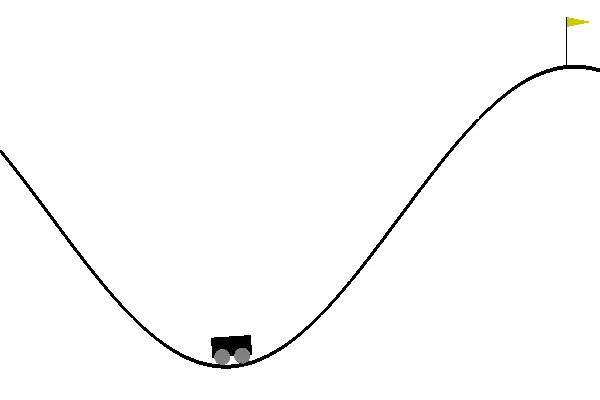
\includegraphics[scale=0.5]{images/domain.jpg}
\end{center}
\caption{Mounting car domain}
\label{domain_image}
\end{figure}
}
\subsection{GYM library}{
As a model of the domain was used GYM library (\url{https://gym.openai.com}), which contain list of environments such as classical "Inverted pendulum swing up" domain, "Atari" computer games, environments with physical world simulation.\par
Each environment communicate with algorithm through observation, action and reward . To process action and obtain new state observation agent must call step() function. As a result, environment returns a tuple with new state observation, reward receiver from environment and boolean episode termination value.
\begin{figure}[h!]
\begin{center}
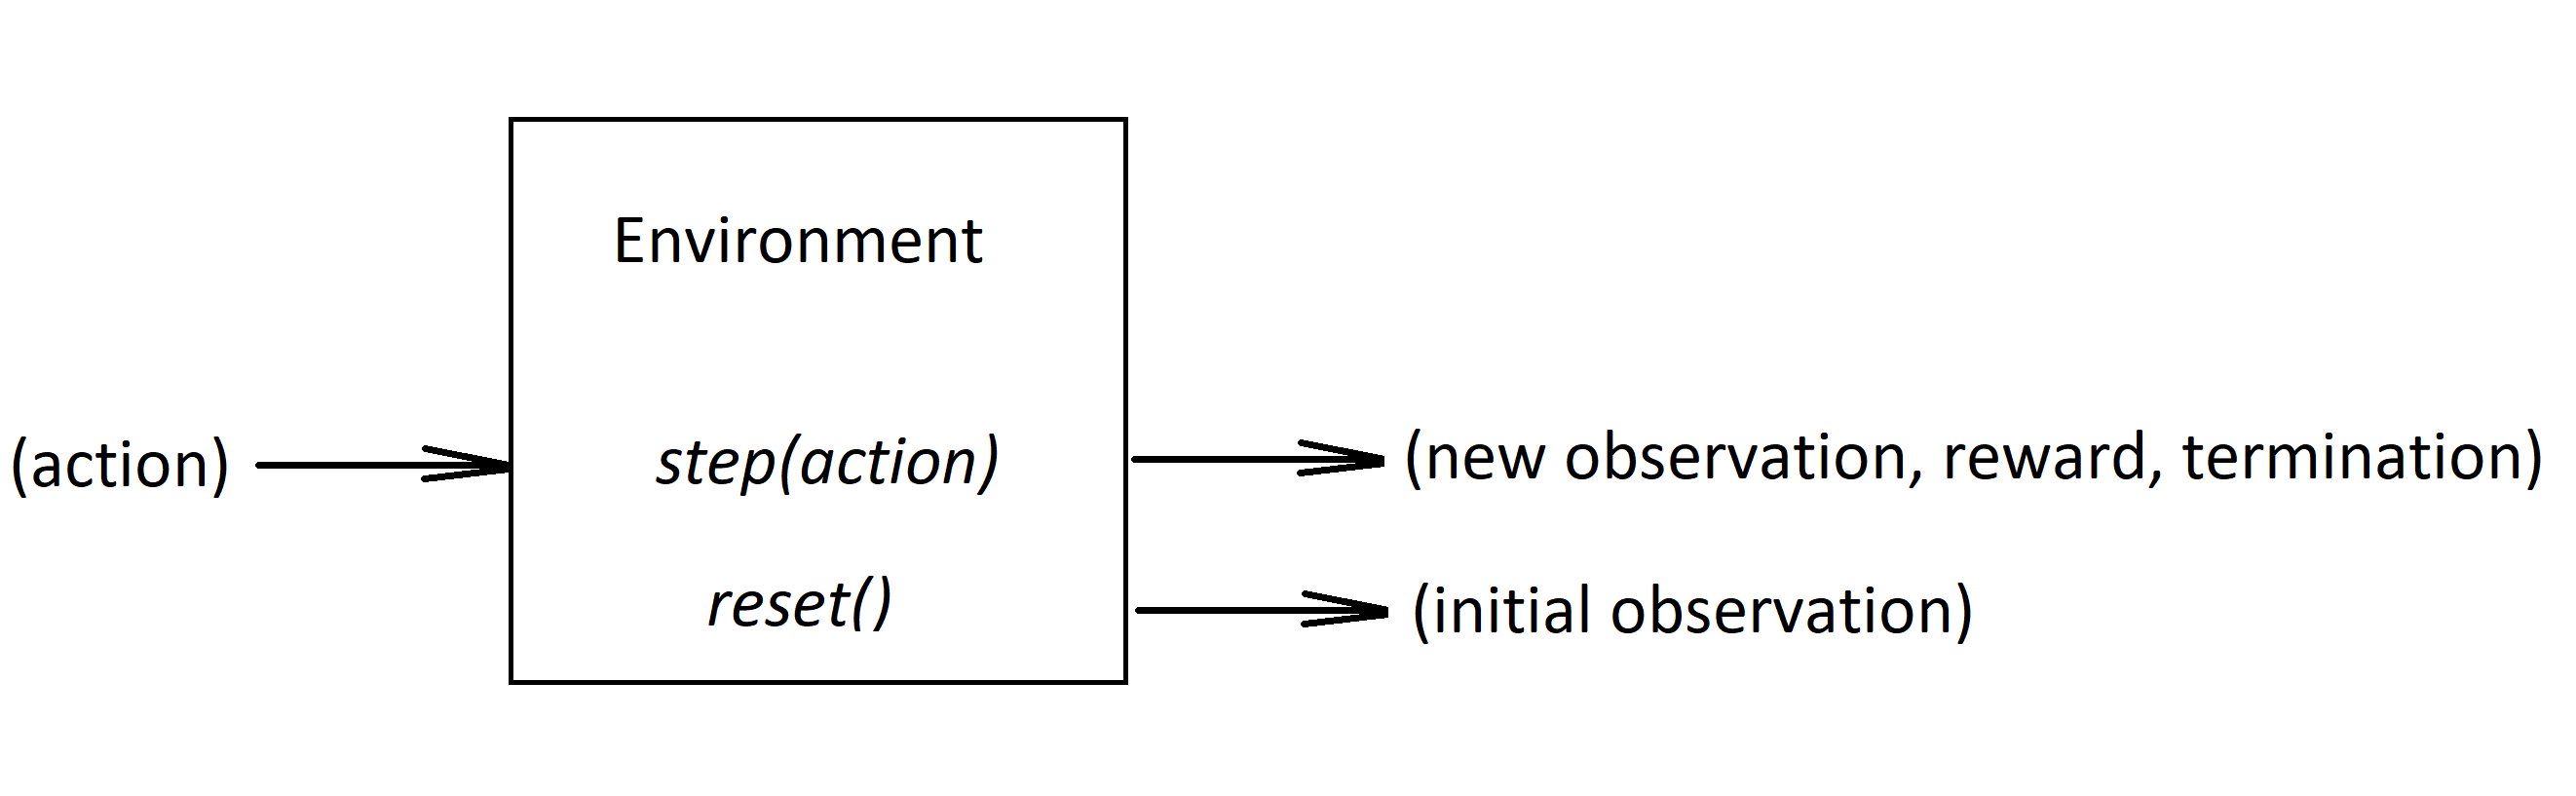
\includegraphics[scale=0.5]{images/gym_env.png}
\end{center}
\caption{GYM environment}
\label{gym_env}
\end{figure}
}
\subsection{Domain specifications}
\label{subsec:spec}{
Each environment in GYM library has different data sizes. For the "Mounting Car" they are:\par
\textit{Observations:} are contain of 2 continuous values of velocity and position:
\begin{center}
$O=\{Vel, Pos\}$,
\end{center}
where $Vel \in [-1.2, 0.6]$ and $Pos \in [-0.07, 0.07]$.\par
\textit{Actions:} are discrete action ids:
\begin{center}
$A=\{0, 1, 2\}$,
\end{center}
where 0 - move back, 1 - no action, 2 - move forward.\par
\textit{Rewards:} are floating point values. Each step, including terminal, gives -1.0 reward.\par
\textit{Termination:} boolean value.
\begin{center}
$T=\{True, False\}$,
\end{center}
where $True$ - termination of episode due to reaching of the goal or taking \textit{200} steps in current episode.\par
}

\newpage
\section{Implementation}
\subsection{Project code structure}{
Code base consist of following classes:
\begin{itemize}
\item \textit{Environment} - wrapper class for GYM environment class
\item \textit{Academy} - class responsible for properly instantiating agent instances, managing training logs, final model saving and restoring.
\item \textit{Agent} - base class for RL agent implementation
\item \textit{Couch} - class that provides methods to train and evaluate agent's performance in the domain
\end{itemize}
}
\subsection{Agents}
\subsubsection{Random Agent}{For comparison and development purposes there was created agent that acts randomly.}
\subsubsection{Look-up table agent}{
To determine value of Q-function for every state-action pair agent use a table of finite size.\par
Since, as desribed in Section~\ref{subsec:spec}, domain has continuous output of speed and acceleration. Thus, observation received from domain discretized into natural numeric value in range [0, 40].\par
In such a way, Q-values table has resulting size of 40x40x3 of floating point values.
}
\subsubsection{Multi-layer perceptron}{
Since domain state observation is continuous values Q-learning can be combined with function approximation. As solution Multi Layer Perceptron (MLP) architecture was selected. Figure~\ref{mlp_model} shows the approximation of the Q-function with MLP for Q-learning.\par
\begin{figure}[h!]
\begin{center}
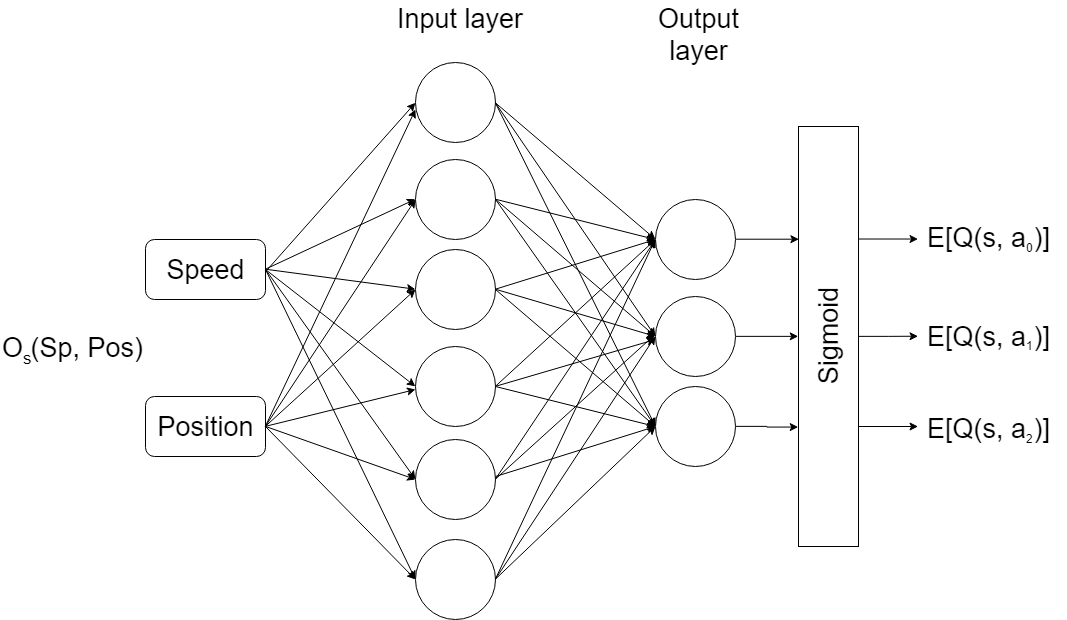
\includegraphics[scale=0.3]{images/mlp_model.png}
\label{mlp_model}
\caption{Q-function approximation model using MLP architecture}
\end{center}
\end{figure}
The learning is based on updating or adjusting the weight matrices of the Neural Network using the equation of the update of the classic algorithm of Q-learning and the algorithm Back propagation.\par
Loss function is determined as squared difference between current state-action utility estimate and updated one:
\begin{center}
$Loss(s, a) = \frac{1}{2}(Q(s, a) - Q'(s, a))^2$,
\end{center}
where $Q'(s, a)$ - updated utility value according to (\ref{q_update}).
}
\newpage
\section{Results}{

}
\newpage
\section{Conclusions}{

}
\newpage
\bibliographystyle{plain}
\bibliography{biblist}



\end{document}
